\documentclass[12pt, a4paper]{article}
\usepackage[a4paper, includeheadfoot, mag=1000, left=2cm, right=1.5cm, top=1.5cm, bottom=1.5cm, headsep=0.8cm, footskip=0.8cm]{geometry}
% Fonts
\usepackage{fontspec, unicode-math}
\setmainfont[Ligatures=TeX]{CMU Serif}
\setmonofont{CMU Typewriter Text}
\usepackage[english, russian]{babel}
% Indent first paragraph
\usepackage{indentfirst}
\setlength{\parskip}{5pt}
% Diagrams
\usepackage{graphicx}
\usepackage{float}
% Page headings
\usepackage{fancyhdr}
\pagestyle{fancy}
\renewcommand{\headrulewidth}{0pt}
\setlength{\headheight}{16pt}
%\newfontfamily\namefont[Scale=1.2]{Gloria Hallelujah}
\fancyhead{}

\usepackage{amsmath}

\usepackage{multirow}

\graphicspath{ {images/} }

\usepackage{listings}
\lstdefinestyle{lablisting}{
  basicstyle=\scriptsize\ttfamily,
  numbers=left,
  stepnumber=1,
  otherkeywords={EOF, O\_RDONLY, STDIN\_FILENO, STDOUT\_FILENO, STDERR\_FILENO},
  numbersep=10pt,
  showspaces=false,
  showstringspaces=false
}

\newcommand{\specialcell}[2][l]{%
 \begin{tabular}[#1]{@{}l@{}}#2\end{tabular}}

\begin{document}

% Title page
\begin{titlepage}
\begin{center}

\textsc{Национальный исследовательский университет ИТМО\\[4mm]
Факультет программной инженерии и компьютерной техники}
\vfill
\textbf{Практическое задание №2\\[4mm]
по дисципение Теория Автоматов\\[4mm]
Минимизация абстрактных автоматов\\[4mm]
}
\textit{Вариант 11\\[16mm]}
\begin{flushright}
Студент: Саржевский Иван
\\[2mm]Группа: P3302
\\[2mm]Преподаватель: Тропченко Александр Ювенальевич
\end{flushright}
\vfill
г. Санкт-Петербург\\[2mm]
2020 г.

\end{center}
\end{titlepage}

\section*{Цель}

Овладение навыками минимизации полностью определенных абстрактных автоматов
(на примере автомата Мура).

\section*{Постановка задачи}

Абстрактный автомат задан табличным способом. Причем абстрактный автомат
Мили представлен таблицами переходов и выходов, а абстрактный автомат Мура - 
одной отмеченной таблицей переходов. Эквивалентные автоматы могут иметь
различное число состояний. В связи с этим возникает задача нахождения минимального
(с минимальным числом состояний) автомата в классе эквивалентных между
собой автоматов. Для минимизации абстрактного автомата использовать алгоритм,
предложенный Ауфенкампом и Хоно. Основная идея алгоритма состоит в разбиении
всех состояний исходного абстрактного автомата на попарно не пересекаемые 
классы эквивалентных состояний. После разбиения происходит замена каждого
класса эквивалентности одним состоянием. Получившийся в результате минимальный 
абстрактный автомат имеет столько же состояний, на сколько классов 
эквивалентности разбиваются состояния исходного абстрактного автомата.

\section*{Исходный граф}

Исходный автомат задается следующей таблицей переходов:

\begin{center}
\begin{tabular}{| c | c | c | c | c | c | c | c | c |}
  \hline
  $\lambda$ & $w_1$ & $w_2$ & $w_2$ & $w_1$ & $w_2$ & $w_2$ & $w_2$ & $w_1$\\
  \hline
  $\delta$ & $a_1$ & $a_2$ & $a_3$ & $a_4$ & $a_5$ & $a_6$ & $a_7$ & $a_8$\\
  \hline
  $z_1$ & $a_5$ & $a_7$ & $a_8$ & $a_5$ & $a_5$ & $a_4$ & $a_6$ & $a_2$\\
  \hline
  $z_2$ & $a_2$ & $a_4$ & $a_8$ & $a_2$ & $a_6$ & $a_2$ & $a_3$ & $a_1$\\
  \hline
\end{tabular}
\end{center}

Графический вид:

\begin{center}
  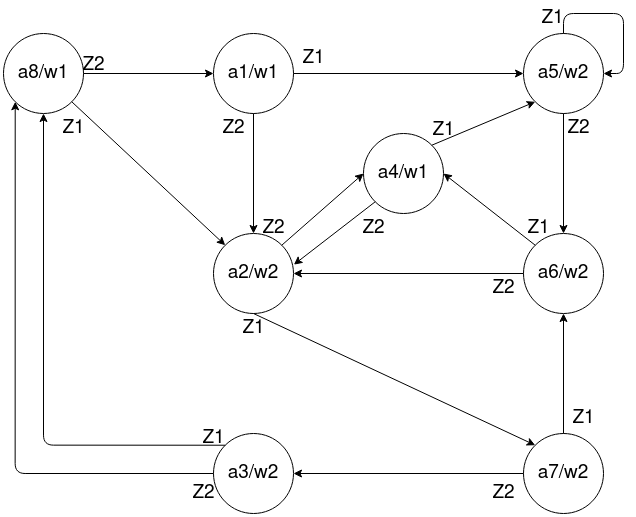
\includegraphics[scale=0.4]{ta2_1}
\end{center}

\section*{Минимизация исходного автомата}

По таблице выходов найдем классы одноэквивалентных состояний.

\noindent
$B_1 = \{a_1, a_4, a_8\}$\\
$B_2 = \{a_2, a_3, a_5, a_6, a_7\}$\\
$P_1 = \{B_1, B_2\}$

\begin{tabular}{| c | c | c | c | c | c | c | c | c |}
  \hline
  \multirow{2}{*}{} & \multicolumn{3}{|c|}{$B_1$} & \multicolumn{5}{|c|}{$B_2$}\\
  \cline{2-9}
  & $a_1$ & $a_4$ & $a_8$ & $a_2$ & $a_3$ & $a_5$ & $a_6$ & $a_7$\\
  \hline
  $z_1$ & $B_2$ & $B_2$ & $B_2$ & $B_2$ & $B_1$ & $B_2$ & $B_1$ & $B_2$\\
  \hline
  $z_2$ & $B_2$ & $B_2$ & $B_1$ & $B_1$ & $B_1$ & $B_2$ & $B_2$ & $B_2$\\
  \hline
\end{tabular}

\noindent
$C_1 = \{a_1, a_4, a_5, a_7\}$\\
$C_2 = \{a_2, a_8\}$\\
$C_3 = \{a_3\}$\\
$C_4 = \{a_6\}$\\
$P_2 = \{C_1, C_2, C_3, C_4\}$\\
$P_1 \ne P_2$ - продолжаем минимизацию.

\begin{tabular}{| c | c | c | c | c | c | c | c | c |}
  \hline
  \multirow{2}{*}{} & \multicolumn{4}{|c|}{$C_1$} & \multicolumn{2}{|c|}{$C_2$} & $C_3$ & $C_4$\\
  \cline{2-9}
  & $a_1$ & $a_4$ & $a_5$ & $a_7$ & $a_2$ & $a_8$ & $a_3$ & $a_6$\\
  \hline
  $z_1$ & $C_1$ & $C_1$ & $C_1$ & $C_4$ & $C_1$ & $C_2$ & $C_2$ & $C_1$\\
  \hline
  $z_2$ & $C_2$ & $C_2$ & $C_4$ & $C_3$ & $C_1$ & $C_1$ & $C_2$ & $C_2$\\
  \hline
\end{tabular}

\noindent
$D_1 = \{a_1, a_4\}$\\
$D_2 = \{a_5\}$\\
$D_3 = \{a_7\}$\\
$D_4 = \{a_2\}$\\
$D_5 = \{a_8\}$\\
$D_6 = \{a_3\}$\\
$D_7 = \{a_6\}$\\
$P_3 = \{D_1, D_2, D_3, D_4, D_5, D_6, D_7\}$\\
$P_2 \ne P_3$ - продолжаем минимизацию.

\begin{tabular}{| c | c | c | c | c | c | c | c | c |}
  \hline
  \multirow{2}{*}{} & \multicolumn{2}{|c|}{$D_1$} & $D_2$ & $D_3$ & $D_4$ & $D_5$ & $D_6$ & $D_7$\\
  \cline{2-9}
  & $a_1$ & $a_4$ & $a_5$ & $a_7$ & $a_2$ & $a_8$ & $a_3$ & $a_6$\\
  \hline
  $z_1$ & $D_2$ & $D_2$ & $D_2$ & $D_7$ & $D_3$ & $D_4$ & $D_5$ & $D_1$\\
  \hline
  $z_2$ & $D_4$ & $D_4$ & $D_7$ & $D_6$ & $D_1$ & $D_1$ & $D_5$ & $D_4$\\
  \hline
\end{tabular}

\noindent
$E_1 = \{a_1, a_4\}$\\
$E_2 = \{a_5\}$\\
$E_3 = \{a_7\}$\\
$E_4 = \{a_2\}$\\
$E_5 = \{a_8\}$\\
$E_6 = \{a_3\}$\\
$E_7 = \{a_6\}$\\
$P_4 = \{E_1, E_2, E_3, E_4, E_5, E_6, E_7\}$\\
$P_3 = P_4$ - завершаем минимизацию.\\
$a_1 \equiv a_4$

\end{document}
